%\documentclass[a4paper,12pt]{article} 
\documentclass[prd,amsfonts,onecolumn,superscriptaddress,aps,nofootinbib,11pt]{revtex4}


\pdfoutput=1
% \usepackage{ae,aecompl}
\usepackage[english]{babel}
\usepackage[utf8]{inputenc}
%\usepackage[latin1]{inputenc}
\usepackage{amsmath,amssymb,mathrsfs}
\usepackage{physics}
% \usepackage{subcaption}
\usepackage{siunitx}
\usepackage{graphicx}
\usepackage{enumerate}
\usepackage{multirow}
\usepackage{float} 
\usepackage[usenames,dvipsnames]{xcolor} 
\usepackage{hyperref}
\hypersetup{colorlinks=true,
		breaklinks=true,
    linkcolor=Blue,          % color of internal links
    citecolor=Plum,        % color of links to bibliography
    urlcolor=YellowOrange           % color of external links
}
\RequirePackage{caption}
%\RequirePackage{subcaption}
\renewcommand{\thesection}{\arabic{section}} 
\renewcommand{\thesubsection}{\thesection.\arabic{subsection}}

\newcommand{\bhat}[1]{\hat{\mathbf{#1}}}

%%%%%%%%%%%%%%%%%%%%%%%%%%%%%%%%%%%%%%%%%%%%%%%%%
\begin{document}
%%%%%%%%%%%%%%%%%%%%%%%%%%%%%%%%%%%%%%%%%%%%%%%%%
\title{{\Large{Trabalho de Conclusão de Curso}}\\ \vspace{0.6 cm}  \large{Emergent electronic states on the Dirac semimetal NiTe$_2$}}


\author{Rodrigo Tardini Paulino}
\email{rodrigo.paulino@aluno.ufabc.edu.br}
\affiliation{Centro de Ci\^encias Naturais e Humanas, Universidade Federal do ABC, Santo Andr\'e-SP, Brasil}

%\author{Colaborador}
%\email{aluno@ufabc.edu.br}
%\affiliation{Centro de Ci\^encias Naturais e Humanas, Universidade Federal do ABC, Santo Andr\'e-SP, Brasil}


%\date{\today}

%%%%%%%%%%% ABSTRACT %%%%%%%%%%%%%%%%%%%%%%%%%%%%%%%%
\begin{abstract}
Escreva aqui o resumo do seu trabalho.   
\end{abstract}
%%%%%%%%%%%%%%%%%%%%%%%%%%%%%%%%%%%%%%%%%%%%%%%%%
\maketitle
%%%%%%%%%%%%%%%%%%%%%%%%%%%%%%%%%%%%%%%%%%%%%%%%%


\section{Introduction} 
\label{sec:intro}


Context:
\begin{itemize}
    \item Topollogically protected states and Weyl/Dirac semimetals
    \item What is a Weyl semimetal?
    \item Why are they of interest to areas of physics such as spintronics and thermoelectricity?
    \item What makes NiTe$_2$ special?
\end{itemize}


Final objectives of the work:
\begin{itemize}
    \item Study the Fermi surface of the Dirac semimetal NiTe$_2$ through the de Haas van Alphen effect
    \item How does the Fermi surface evolves with Se substitution on the Te site?
    \item Are the Dirac cones altered? Do we change the location of the Dirac points? Can this me observed through the de Haas-van Alphen effect?
\end{itemize}






\section{The de Haas-van Alphen effect}
\label{sec:dHVa}


\begin{itemize}
    \item Historical introduction (Landau, Onsager, de Haas, van Alphen)
    \item Simplified Landau model for free electrons (explain the concept of Landau tubes)
    \item Onsager's relation between the period of the oscilations and the Fermi surface
    \item The basics of the Lifshitz-Kosevich formula (how much detail is needed? Just cite the reference and show the results?)
\end{itemize}



\subsection{Landau levels in free electrons}



In order to understand the full phenomena, let's first take a closer look on the simpler case of the free electrons under a constant magnetic field $H$.

Just as in the case of classical physics, the initial Hamiltonian that describes free particles of charge $e$ under a magnetic field is given by
\begin{equation}
    \bhat{H} = \frac{\bhat{p} - e\vb{A}/c}{2 m}
\end{equation}
, where $\bhat{p}$ is the momentum operator $\bhat{p} = -i \hbar \grad$, and $\vb{A}$ is the vector potential of the magnetic field. But since this comes from the classical picture, the quantum mechanical effects needs to take into acount the intrinsic magnetic moment $\bhat{\mu}$ of the particles that couples with the external field, that is written in the form of
\begin{equation}
    \bhat{\mu} =\frac{\mu \bhat{s}}{s}
\end{equation}
where $\bhat{s}$ is the spin operator, and $\mu$ is a constant that characterises the particle ($\mu = 1/2$ for the electron). For the porpuse of this work, we don't need to take other effects such as spin-orbit coupling into account, which would result on the Zeeman effect as well.

So the Hamiltonian for the free electron under a magnetic field $H$ becomes
\begin{equation}
    \bhat{H} = \frac{(\bhat{p} - e\vb{A}/c)^2}{2 m} - \bhat{\mu}\cdot H
\end{equation}

In order to determine what are the energy levels of these particles, we can orient the magnetic field on the $\hat{z}$ direction, and using the gauge invariance of the magnetic field, the vector potential is taken to be $\vb{A}=-H y \bhat{x}$.

This vector potential is chosen in a way that it commutes with the momentum operator, meaning that the final hamiltonian can be simplified to 
\begin{equation}
    \bhat{H} = \frac{1}{2 m}\left(\hat{p}_x + \frac{e H y}{c}\right)^2 + \frac{\hat{p}_y^2}{2m} + \frac{\hat{p}_z^2}{2m} - \frac{\mu}{s}\hat{s}_z   H
\end{equation}



Since we do not have any spin components other than $\hat{s}_z$, the hamiltoniam commutes with this operator. The same happens for the $\hat{p}_x$ and $\hat{p}_z$, because the operators $\hat{x}$ and $\hat{z}$ are not present. Therefore, this are all conserved quantities. 

The first consequence, is that the spin eigenvalue can be taken as a constant $s_z = \sigma = \pm 1$, and the eigenfunction  $\psi$ of the hamiltonian can be considered an ordinary coordinate function, resulting in
\begin{equation}\label{eq:schrodinger}
    \frac{1}{2m} \left[ \left(\hat{p}_x + \frac{e H y}{c}\right)^2  + \hat{p}_y^2 + \hat{p}_z^2 \right]\psi - \frac{\mu}{s} \sigma H \psi = \epsilon \psi
\end{equation}

Since the $x$ and $z$ coordinates of the generalized momentum are conserved, we can use separation of variables to show that the eigenfunction we look for is in the form
\begin{equation}\label{eq:psi}
    \psi = \chi(y) e^{\frac{i}{\hbar}(x p_x + z p_z) }
\end{equation}
, this can then be substituted back on equation \ref{eq:schrodinger}, considering that the operators $\hat{p}_i = -i \hbar \dv{}{x^i}$ since the eigenfunction is in the coordinate basis

\begin{equation}
    \frac{1}{2m} \left[ \chi \dv[2]{}{x} e^{\frac{i}{\hbar}x p_x}
+ \dv[2]{}{y}\chi
+ \chi \dv[2]{}{z} e^{\frac{i}{\hbar}z p_z }
- i \hbar \left(\frac{e H y}{c}\right) \chi \dv{}{x} e^{\frac{i}{\hbar}x p_x}    + \left(\frac{e H y}{c}\right)^2\chi    \right] - \frac{\mu}{s} \sigma H \chi = \epsilon \chi
\end{equation}
which can then be simplified to
\begin{equation}
        \frac{1}{2m} \left[ -\frac{1}{\hbar^2} p_x^2 \chi
+ \chi''
+ -\frac{1}{\hbar^2} p_z^2 \chi
+  \frac{e H y}{c} p_x \chi   + \left(\frac{e H y}{c}\right)^2\chi    \right] - \frac{\mu}{s} \sigma H \chi = \epsilon \chi
\end{equation}
and finally
\begin{equation}\label{eq:simplified}
    \chi'' + \frac{2m}{\hbar^2} \left(  \epsilon + \frac{\mu \sigma}{s}H - \frac{p_z^2}{2m} - \frac{1}{2} m \left( \frac{e H}{mc}   \right)^2 \left[y - \left( - \frac{c p_x}{e H}  \right)\right]    \right) \chi = 0
\end{equation}
.


The equation \ref{eq:simplified} is identical to the solution of Schrodinger's equation for the harmonic oscilator
\begin{equation}\label{eq:oscilator}
    \chi'' + \frac{2m}{\hbar^2} \left[  \epsilon + \frac{\mu \sigma}{s}H - \frac{p_z^2}{2m} - \frac{1}{2} m \omega_H^2 \left( y - y_0\right)    \right] \chi = 0
\end{equation}
, where the frequency is $\omega_H = \frac{e H}{mc}$ and the central coordinate on the $y$ direction is $y_0 = \frac{-c p_x}{eH}$. Using the result of the harmonic oscilator, considering that the spin magnetic moment $\mu_B = \frac{e\hbar}{m}$ for the electron leads to $\frac{\mu}{s} = \frac{-e \hbar}{mc}$ , the energy becomes
\begin{equation}
    \epsilon(n, k_z) = \frac{\hbar^2 k_z^2}{2m}  + \hbar \omega_H  \left( n + \frac{1}{2} + \sigma \right)
\end{equation}
, and the eigenfunction is
\begin{equation}
    \chi_n(y) = \frac{1}{\sqrt{\pi^{1/2} a_H (2^n n!)}} exp \left[ - \frac{(y - y_0)^2}{2 a_H^2} \right] H_n\left( \frac{y - y_0}{a_H}  \right)
\end{equation}
where $H_n$ are the Hermite polynomials of order $n$, and $a_H = \sqrt{\frac{\hbar}{m \omega_H}}$. 

The states with a given value of $n$ are known as Landau levels.

This eigenfunction can be looked at a similar form to the classical picture of the cyclotron orbit of the electron, where the momentum in the direction of the field can take any value, and the electron has a "circular orbit" on the $xy$ plane with the cyclothron frequency $\omega_H = \frac{e H}{mc}$. Since the z-coordinate is not influenced by the field, the semi-classical orbit of the electron has a cyllindrical form, called the Landau tubes.


An important result here is that the energy levels, that are continous in the case of free electrons, are quantized when an external magnetic field is applied, with the cyclothron frequency and the energy spacing of the Landau levels increasing linearly with $H$.

The next step is to determine the degeneracy of each of this Landau levels. For this, consider the electron is at the fundamental state, confined in a box of size $L_x$, $L_y$ and $L_z$.


The first consequence comes in the x-coordinate by the boundary condition of the wavefunction in equation \ref{eq:psi}, where 
\begin{equation}
    k_x = \frac{2 \pi }{L_x}m
\end{equation}
, where $m$ is an integer. The value of $m$ is further restricted when you consider the quantity $y_0 = \frac{c \hbar k_x}{e H}$, that can be thought as the y-coordinate for the center of the oscilattory wavefunction. Since this center must physically lie within the system ($0\leq y_0 < L_y $) resulting on
\begin{equation}
    k_x < \frac{e H L_y}{c \hbar}
\end{equation}
which can then be combined to 
\begin{equation}
    0 \leq m < \frac{e H L_x L_y}{2 \pi c \hbar} .
\end{equation}

The degeneracy of the Landau levels is given when $m$ is maximum,
\begin{equation}\label{eq:degeneracy}
    \eta = \frac{A H}{\phi_0}
\end{equation}
, where $H$ is the field, $\phi_0 = \frac{hc}{2e}$ is the flux quanta, and $A$ is the area of the box, that will be taken as the Fermi surface's extremal area in solids.


Notice that the degenaracy of the Landau level increases with applied field. This effect, combined with the different energies of each Landau levels, will leed to an oscillatory behaviour on the energy, and is the origin of the de Haas-van Alphen oscillations. 


\subsection{The periodicity of the oscillations}

When a magnetic field is applied, the levels $n = 0,1,2, ... , k-1$ will be fully occupied with $\eta$ electrons each, while the level $n=k$ will pe partially occupied with $\lambda \eta$ electrons. Thus we have $N = \eta(k + \lambda)$ electrons, and using equation \ref{eq:degeneracy}

\begin{equation}\label{eq:filling}
    k + \lambda = \frac{N \phi_0}{A} \frac{1}{H} = \frac{N h c}{2 e A} \frac{1}{H} = \frac{H_0}{H},
\end{equation}
where $H_0 = \frac{N \phi_0}{A}$ is the minimum field required to to put all the electrons in the lowest Landau level.

Notice that $k$ is an integer value and $\lambda \in [0,1)$, so we can define 
\begin{align}\label{eq:coefs}
    k = \left[ \frac{H_0}{H}   \right], && \lambda = \frac{H_0}{H} - \left[ \frac{H_0}{H}   \right],
\end{align}
where $[x]$ represents the integer value of $x$.

The energy of the system is obtained by summing the energy of each electrons, and by considering that the overall contribution of spin is cancelled out

\begin{align}
    E(H) &=  \eta \hbar \omega_H   \left[\sum_{n=0}^{k-1} ( n + \frac{1}{2}  )  + ( k + \frac{1}{2} )\lambda \right]  \\
    &= \eta \hbar \omega_H \left[ k \left(\frac{k-1}{2}  + \frac{1}{2}\right)   +  ( k + \frac{1}{2} )\lambda  \right] \\
    &= \eta \hbar \omega_H \left[   \frac{k^2}{2}  + (k + \frac{1}{2})\lambda       \right] \\
    &= \eta \hbar \omega_H \left[ \frac{(k + \lambda)^2}{2}  + \frac{\lambda - \lambda^2}{2}   \right] \\
    &= N \hbar \omega_H \left[ \frac{k + \lambda}{2}   + \frac{\lambda(1-\lambda)}{2(k+\lambda) }    \right] \\
    &= \frac{N^2 \pi \hbar^2 }{2 m A} + \frac{N \hbar \omega_H}{2(k+\lambda)} \lambda(1 - \lambda), 
\end{align}
and considering that the energy at field 0 is

\begin{equation}\label{eq:E(H=0)}
    E(H=0) = N\frac{\epsilon_f}{2} = \frac{N^2}{A} \frac{\pi \hbar^2}{2 m} 
\end{equation}
the energy can be represented in a much simpler form
\begin{equation}\label{eq:energy}
    \frac{E(H)}{E(H=0)} = 1 + \left( \frac{H}{H_0} \right)^2 \lambda(1-\lambda) .
\end{equation}

From equation \ref{eq:energy}, it can be seen that the energy of the system increases with $H^2$, and most importantly, equation \ref{eq:coefs} shows that $\lambda$ goes to 0 periodically with $\frac{1}{H}$, and the energy follows that oscillation pattern.

Since the magnetization is defined as
\begin{equation}
    M = - \pdv{E}{H},
\end{equation}
than the magnetization will also oscillate with a constant period at $\frac{1}{H}$
\begin{equation}
    \Delta\left( \frac{1}{H} \right) = \frac{1}{H_0} = \frac{2 e A}{h c N}.
\end{equation}

In order to further simply this relation, consider the Fermi energy of the free electron and the wave vector  $E_f = \frac{N}{A}\frac{\pi \hbar^2}{m} = \frac{\hbar^2 k_f^2}{2m}$ and defining the Fermi area $A_f = \pi k_f^2$
\begin{equation}
    \Delta\left( \frac{1}{H} \right) = \frac{2 \pi e}{\hbar c} \frac{1}{A_f}.
\end{equation}


This area is fixed for a given number of electrons, but the amount of Landau tubes that fit this area changes depending on the applied field. The radius of this semiclassical Landau tube of the level $p$ is 
\begin{equation}\label{eq:periodicity}
    \frac{\hbar^2 k_p^2}{2m} = (p + \frac{1}{2})\hbar \omega_H \Rightarrow k_p^2 = (p + \frac{1}{2}) \frac{2 \pi e H}{\hbar c},
\end{equation}
and because of this result, the oscilations can be seen as the "popping out" of the Landau tubes of the Fermi area.

Even though this was deduced for the case of free non-relativistic electrons, it can be shown that Dirac fermions on metals exibit the exact same periodicity  relation as the equation \ref{eq:periodicity}, where $A_f$ is the extremal area of the Fermi surface perpendicular to the applied field. CITE ONSAGER 

\subsection{General form of oscillations}

The experimentally studied material is always under a finite temperature, resulting in different filling of the Landau levels as previously discussed in equation \ref{eq:filling}. Fermi-Dirac statistics would introduce an energy close to $k_B T$, supressing the Landau splitting depending on its energy value. Based on this principle, the first condition for the de Haas-van Alphen effect is
\begin{equation}
    \hbar \omega_G = \frac{e \hbar}{mc} H \gg k_B T.
\end{equation}
Notice that this inequality requires both a large magnetic field, and a low temperature.




The second condition comes from the impurities on the crystalline lattice. The finite lifetime $\tau$ will broaden the energy levels by $\frac{\hbar}{\tau}$ 
\begin{equation}
    \hbar \omega_H \gg \frac{\hbar}{\tau} \Rightarrow \tau \omega_H \gg 1.
\end{equation}


For this reason, the equation that describes the oscillations on the magnetization should come directly from a quantum statistics framework. This was first developed by Lifshitz-Kosevich DATE AND REFERENCE, and further adapted to relativistic fermions and different dimensionalities. REFERENCES

The revised Lifshitz-Kosevich formula is
\begin{equation}
        \Delta M \propto -B^{\lambda} R_T   R_D   R_S  \text{ sin}\left[ 2\pi \left( \frac{F}{B} - \frac{1}{2} + \frac{\Phi_B}{2 \pi} - \delta  \right)      \right],
\end{equation}
where $R_T = \frac{\alpha T \mu / B  }{\text{sinh}[\alpha T \mu / B ]}$, $R_D =  \text{exp}[ -\alpha T_D \mu / B ]$, $R_S = \text{cos}(\pi g \mu /2 )$. $\mu = m^*/m_0$, $\alpha = 2 \pi^2 k_B m_0 / \hbar e$ and $T_D$ is the Dingle temperature. Both the thermal $R_T$ and the Dingle $R_D$ damping factors come from the broadening of the Landau levels, caused by temperature on the Fermi-Dirac distribution and electronic scattering, respectively. $R_S$ is the constant spin reduction factor due to Zeeman splitting. 

The oscillation of the magnetization comes from the sine function, with the aditional Berry phase $\Phi_B$ and a dimensional phase $\lambda = 0 (\pm \frac{1}{8})$ for 2D(3D) Fermi surfaces. The field exponent in the amplitude $\lambda$ is also dimensionally dependent, with $\lambda = 0 (\frac{1}{2})$ for 2D(3D) systems.

Therefore, the de Haas-van Alphen effect is able to obtain not only the extremal area of the Fermi surface, but also the Dingle temperature ($R_T$), the band effective mass $m^*$, the quantum relaxation time $\tau_q$ and the quantum mobility $\mu_q$, with the following equations: 
\begin{align}
    \tau_q = \frac{\hbar}{2 \pi k_B T_D}, && \mu_q = \frac{e \tau_q}{m*}.
\end{align}


 

\section{Experimental procedures}
\label{sec:experimentos}

\begin{itemize}
    \item Growth of single crystalline samples
    \begin{itemize}
        \item Flux method
        \item Phase diagrams
    \end{itemize}
    \item Structural characterizations
    \begin{itemize}
        \item X-Ray diffraction
        \item Pattern analysis: FullProf Suite and AutoFP
        \item Energy dispersive X-Ray spectroscopy
    \end{itemize}
    \item Resistivity measurenments
    \item Magnetic characterization
    \begin{itemize}
        \item Superconducting Quantum Interferometer Device (SQUID) on the MPMS
        \item AC Measurement System on the PPMS
        \item Data analysis on Python. FFT, least squares
    \end{itemize}
\end{itemize}

\subsection{Single crystal synthesis}

Condensed matter physics is focused on the study of macroscopic manifestation of delicate quantum phenomena, such as superconductivity and magnetism, that requires high quality samples as a starting point for any experimental work in the area. The visualization of such effects are usually highly dependent on the crystallographic direction and might be suppressed by impurities in the lattice, well exemplified in the de Haas-van Alphen effect described on section \ref{sec:dHVa}.

By growing the material in a single-crystalline form, these extrinsic factors (i.e. impurities, grain boundaries, secondary phases) can be minimized, while enabling the study of orientation dependent properties. This session is aimed at explaining the flux method used for obtaining the NiTe$_2$.

The flux method consists on providing a stable liquid environment for the reagents to be dissolved and later crystallized on the desired phase upon cooling. Usually, the flux is a metallic element with a low melting point and few stable compounds with the reagent, but in the case of NiTe$_2$, a self-flux method was used, where Te is not only on the compound, but is also the flux.

An advantage of flux growths can be easily seen by considering that Ni can be easily dissolved in liquid Te (above Te's melting point at $T_f = 450 $ CELSIUS), reducing the required temperature drastically from Ni's melting point at $T_f = 1455$ CELSIUS. The proportion of Te to the other reagents will determine what phase is the most stable thermodinamically [REFERENCE ASM], and by cooling it slowly from high temperatures, the crystallization will occur in fewer nucleation sites, reducing the number of crystals, but increasing their size and crystallographic purity. The major disadvantage is that the excess reagent can sometimes constitued impurity layers inside the single crystal, but the observation of the de Haas-van Alphen effect indicates that this is not the case of NiTe$_2$. 


Following REFERENCE XU, about 10g (CONFIRM) of reagents at a molar proportion of Ni:Te at 1:8 was used systematically to obtain NiTe$_2$ samples (instead of the stoichiometric 1:2 ratio). Other proportions, with 90, 92 and 94\% of Te were tested, but no significant improvement was found. For the Se chemical substitution, Se was considered to enter the flux together with Te, so a 5\% substitution (NiSe$_{0.1}$Te$_{1.9}$) was grown using the proportion of the Ni:Se:Te at 1:0.4:7.6.

The reagents used were all made by Alfa Aesar (REFERENCE) with high purity (99.9999\% for Te, 99.999\% for Se and 99.95\% for Ni). After careful weighting, the elements were sealed under vacuum in a quartz tube with some quartz wool on top, that will later be used for separation of the flux and the crystals. The setup can be visualized in figure \ref{fig:exp:ampole}.











\begin{figure}[H]
    \centering
    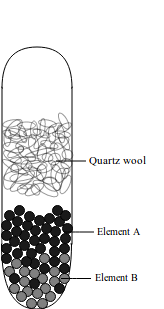
\includegraphics[width=0.15\textwidth]{experiments/Ampole.png}
    \caption{Ampoula}
    \label{fig:exp:ampole}
\end{figure}



\begin{figure}[H]
    \centering
    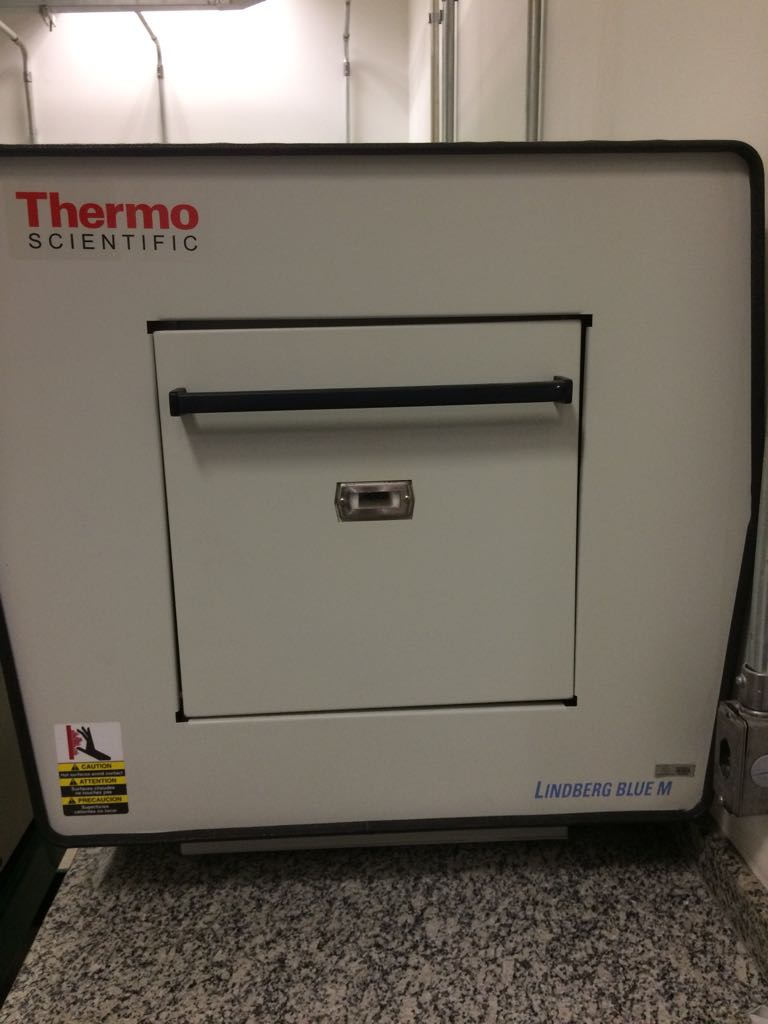
\includegraphics[width=0.4\textwidth]{experiments/forno_mufla.jpeg}
    \caption{Forno de Mufla}
    \label{fig:exp:forno}
\end{figure}



\begin{figure}[H]
    \centering
    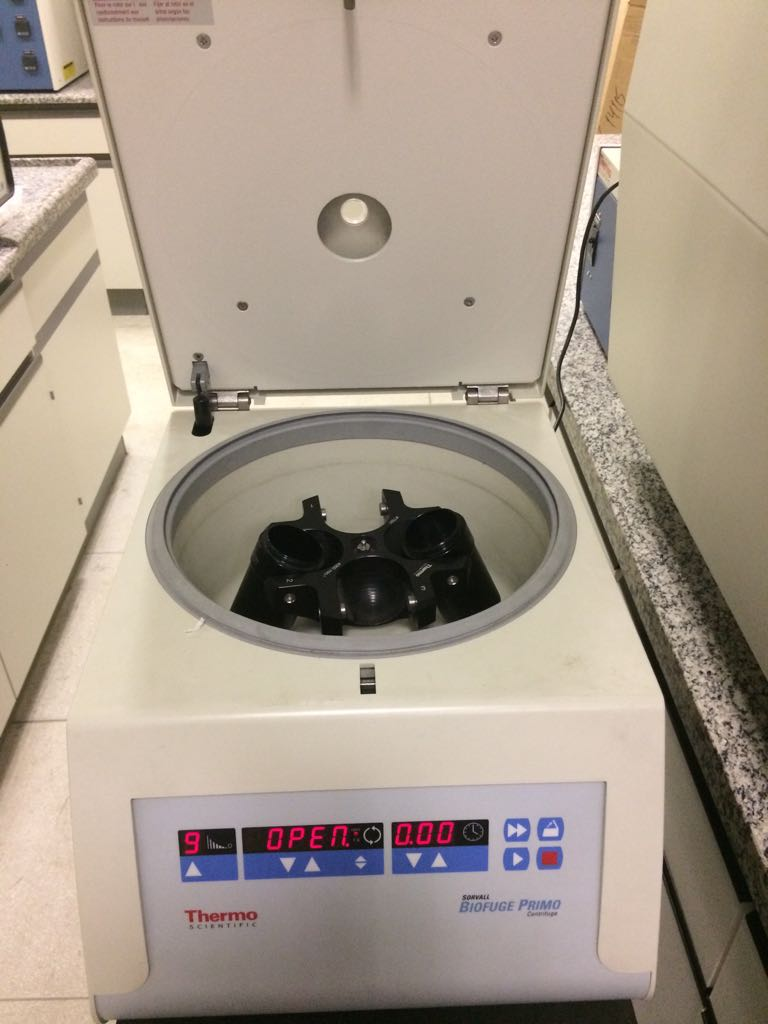
\includegraphics[width=0.4\textwidth]{experiments/centrifuga.jpeg}
    \caption{Centrifuga}
    \label{fig:exp:centrifuga}
\end{figure}

\subsection{Structural characterizations}

\begin{figure}[H]
    \centering
    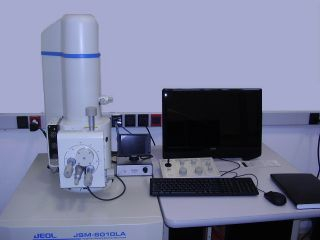
\includegraphics[width=0.4\textwidth]{experiments/MEV_compacto0.jpg}
    \caption{MEV Compacto}
    \label{fig:exp:MEV}
\end{figure}


\subsection{Electronic and magnetic characterization}

\begin{figure}[H]
    \centering
    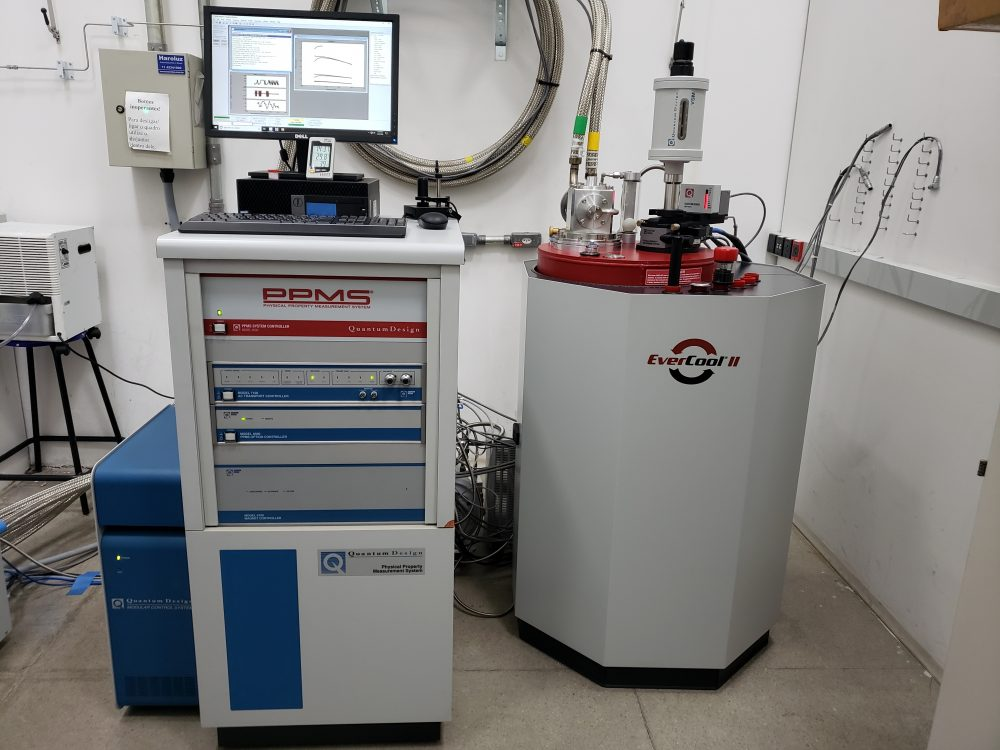
\includegraphics[width=0.4\textwidth]{experiments/PPMS.jpg}
    \caption{PPMS}
    \label{fig:exp:ppms}
\end{figure}


\begin{figure}[H]
    \centering
    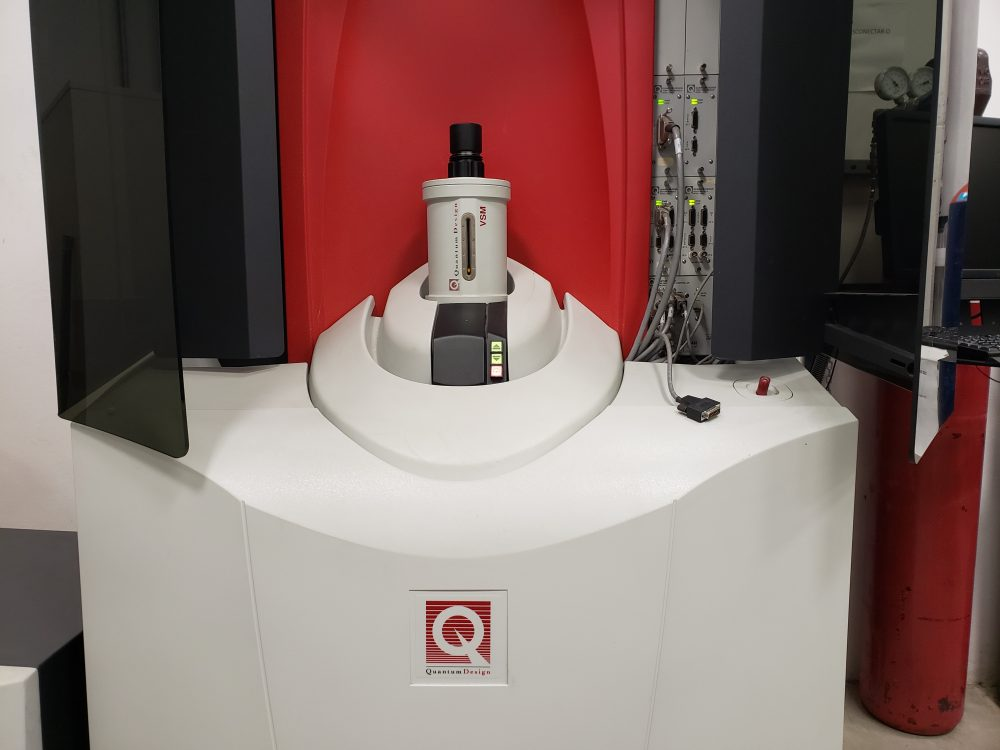
\includegraphics[width=0.4\textwidth]{experiments/SQUID.jpg}
    \caption{SQUID}
    \label{fig:exp:squid}
\end{figure}




\section{Results and discussion}\label{sec:resultados}

\begin{itemize}
    \item Confirmation of the structure
    \item Metalicity of the sample through the resistivity and the magnetization
    \item MxH, and the de Haas-van Alphen oscillations
    \begin{itemize}
        \item Obtaining the oscillation frequencies
        \item Fermi surface area perpendicular to the magnetic field direction
        \item Dingle temperature
        \item Mobility and quantum lifetime of the charge carriers
    \end{itemize}
\end{itemize}


\begin{figure}[H]
    \centering
    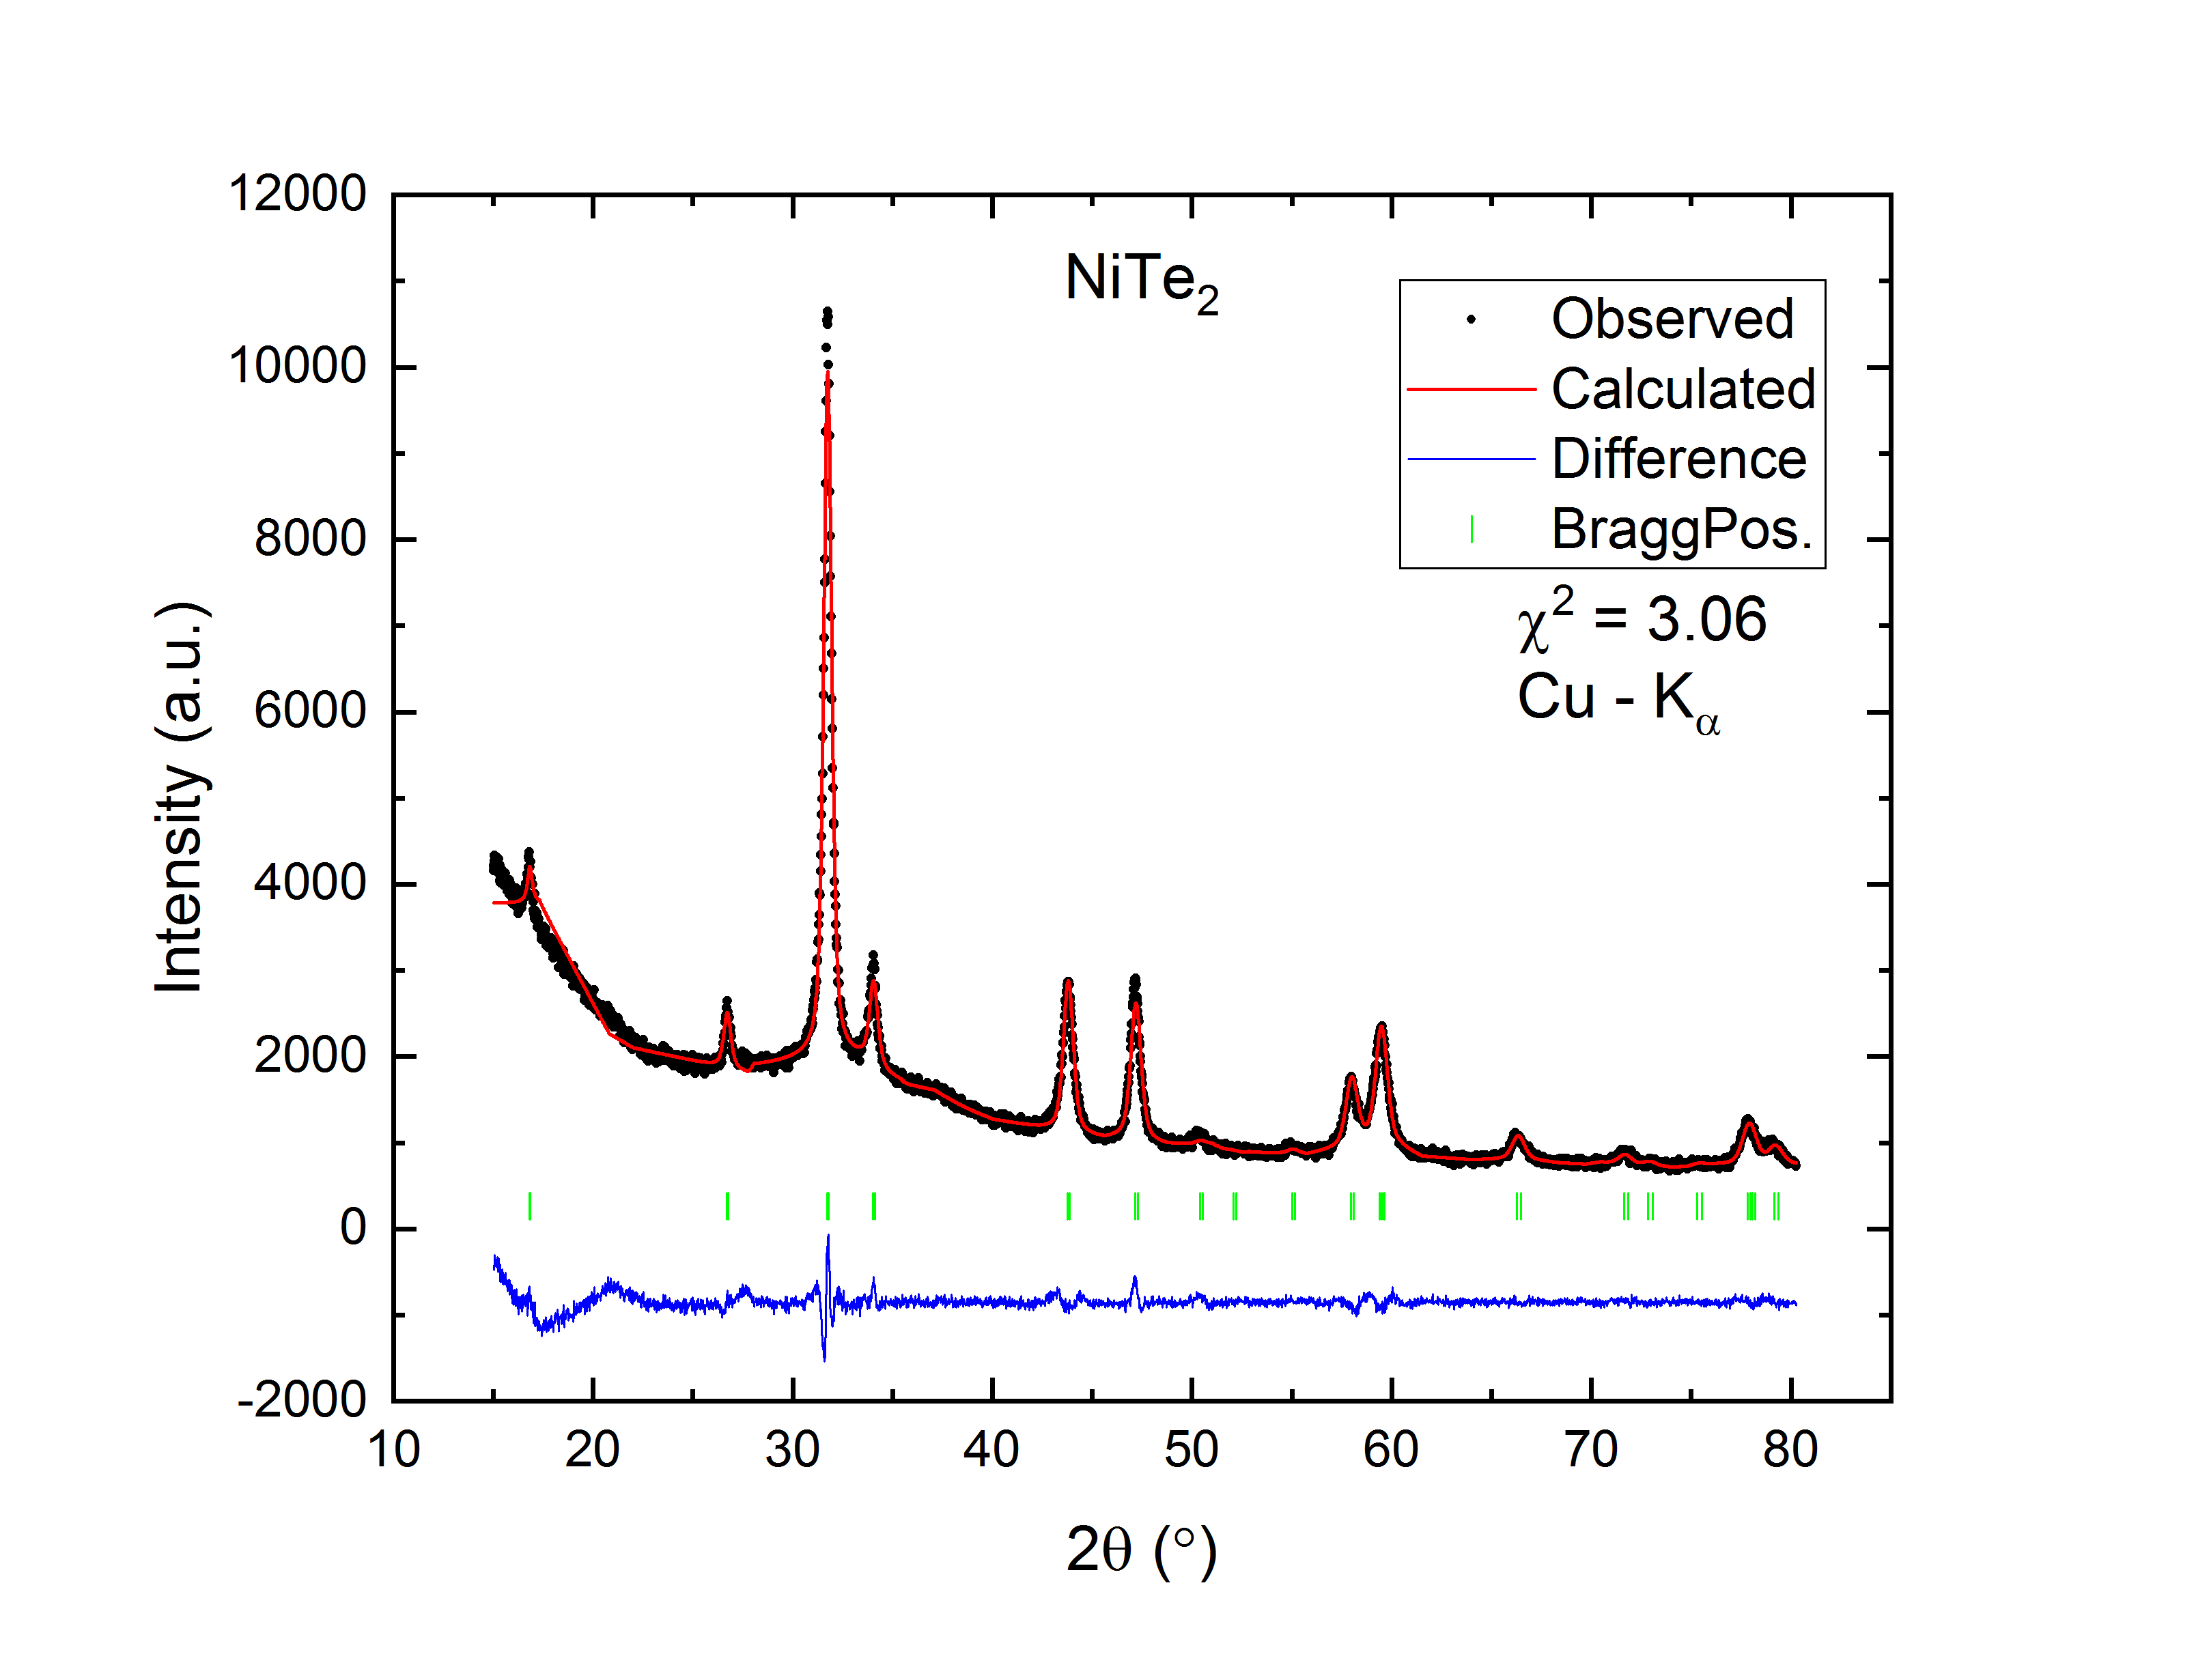
\includegraphics[width=0.4\textwidth]{results/DRX_GMQ632a.png}
    \caption{Difracao de raios-X do NiTe2}
    \label{fig:drx}
\end{figure}

\begin{figure}[H]
    \centering
    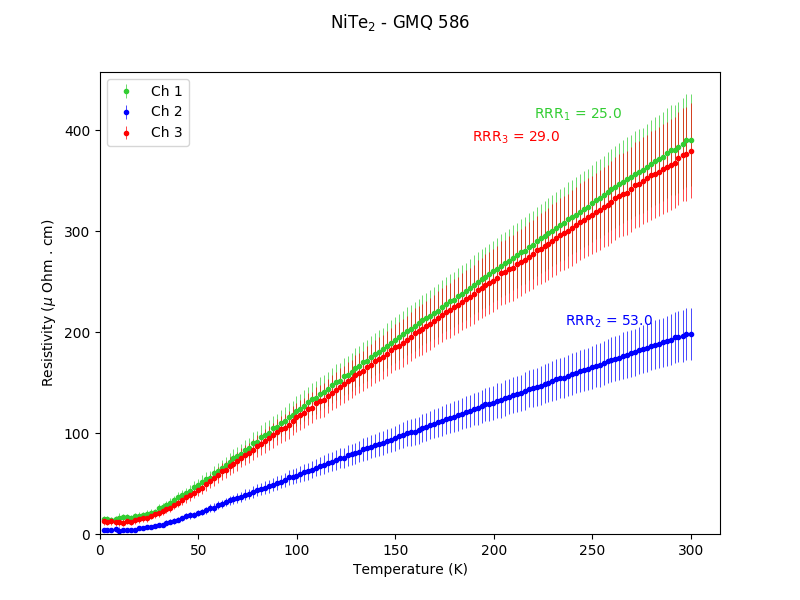
\includegraphics[width=0.4\textwidth]{results/Resistivity.png}
    \caption{Resistivity}
    \label{fig:rho}
\end{figure}



\begin{figure}[H]
    \centering
    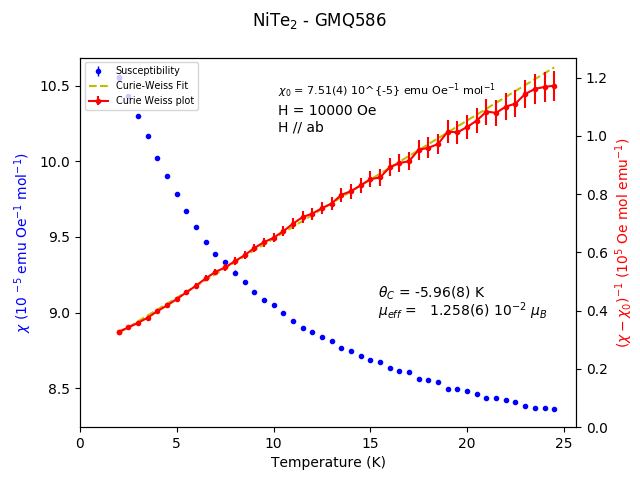
\includegraphics[width=0.4\textwidth]{results/GMQ586-chi-curieweiss.png}
    \caption{Susceptibilidade e o ajuste pela Curie Weiss}
    \label{fig:suscep}
\end{figure}




\section{Conclusions }
\label{sec:conclu}
\section{Results and discussion}\label{sec:resultados}
\newpage


\appendix


\section{Introdução} 


O primeiro passo para começar o seu Trabalho de Conclusão de Curso (TCC) é ter um tema de sua familiaridade, i. e., que você já pesquisou sobre ele. O TCC pode ser sobre: 

-- Uma revisão de um problema na física que já foi estudado por outros pesquisadores e que 
ainda desperta interesse na comunidade científica. 
Por exemplo, apesar do fato da existência de buracos negros ter sido consolidada  
no final da  década de 30 como uma previsão da teoria da relatividade geral ,  tais objetos têm levado a diversos avanços e questões 
desafiadoras nos campos teórico, observacional e experimental. Um TCC que propõe uma revisão 
deve apresentar os principais desenvolvimentos na literatura, incluindo  
o estado atual das pesquisas sobre tema. Em um TCC com essa proposta não são espera resultados 
originais mas sim um estudo que pode dar ao leitor as principais ideias dos problemas e desafios 
envolvidos no tema pesquisado. 

-- Um trabalho de pesquisa que você tem realizado e que contenha resultado original. Se você 
fez ou faz iniciação científica o estudo feito e seus resultados podem ser apresentados como 
um TCC. 

Como sugestão, você pode por provisóriamente a primeira ideia de estrutura
do seu trabalho. Por exemplo, um TCC sobre matéria poderia ter a seguinte
organização de estudo:
\begin{itemize}
\item Dar a ideia de como surgiu o problema da matéria escura falando sobre
as primeiras evidências indiretas em aglomerados de galáxias
e observações das curvas de rotação de galáxias .
Alguns artigos recentes de revisão sobre o tema são .
A história do problema da matéria escura pode ser vista, por exemplo,
em.
\item Mencionar as referências atuais que trataram do tema estudado, e que
eventualmente estejam relacionados a ele. 
\item Apresentar os desenvolvimentos que você realizou. Isso pode ser uma
revisão organizada sobre o tema de estudo ou uma pesquisa que você
realizou na iniciação científica, por exemplo.
\item Apresentar as conclusões do seu estudo.
\end{itemize}

Dicas interessantes para uma boa escrita de trabalhos científicos
são dadas no artigo de \href{https://www.nature.com/articles/d41586-019-02918-5?utm_source=Nature+Briefing&utm_campaign=c699f7417d-briefing-dy-20190927&utm_medium=email&utm_term=0_c9dfd39373-c699f7417d-43483813}{Van Savage e Pamela Yeh}
publicado na Career Columm da Nature.

Sobre o processo de escrita do TCC, deixe a introdução para ser feita no final. 

Você pode escrever seu TCC em inglês se você tiver fluência suficiente nessa língua.

Na Introdução apresente ao leitor o tema de estudo contando sobre
os avanços essenciais da área que levaram ao tema do seu trabalho.
Cite os artigos principais e outras fontes -- que podem
ser livros -- procurando manter ordem cronológica dos fatos.
Esse tema pode ser um problema particular que você irá tratar, ou
uma revisão que você sobre um assunto con a finalidade de se atualizar
sobre os desenvolvimentos recentes e considerados importantes --
\emph{o estado da arte} -- do tema que você pesquisou.

A motivação do seu trabalho deve ser colocada aqui também. 

Indique o que será feito a seguir. Por exemplo, você pode dizer no último parágrafo 
da Introdução algo como: 

O trabalho está organizado da seguinte forma. Na Seção  fazemos 
uma breve revisão sobre os desenvolvimentos experimentais/teóricos/computacionais essenciais 
para nosso trabalho. Na Seção apresentamos o modelo 
a partir do qual realizaremos nossos cálculos. Na Seção 
mostramos o método utilizado 
e nossas análises. Nossas conclusões são apresentadas na Seção .



\section{O efeito de Haas-van Alphen}




Introduza ao leitor às equações, definições, ferramentas matemáticas
que você julga serem necessárias para o bom entendimento do leitor
que não é um especialista na área. Tente apresentar de forma simples
-- o que não significa trivial -- e clara. Em
geral, um leitor poderá ver a partir daqui conceitos que não lhe são
familiar e ficará grato se você explicar bem. Em um apêndice pode
ser colocado ainda por algo mais técnico que não é crucial para seguir
a leitura. Por exemplo, a dedução de um resultado utilizado em seu
desenvolvimento pode ir para o apêndice (veja a mostração desse resultado
no. Se o resultado melhor citar uma referência onde
a mostração do resultado é feita. 



%\newpage
%\section*{References} 

%\bibliographystyle{JHEPfixed}
%\bibliographystyle{JHEP}
\bibliographystyle{apsrev4-1} 

\bibliography{referencias}

%\begin{thebibliography}{99}


%\end{thebibliography}



%%%%%%%%%%%%%%%%%%%%%%%%
\end{document}
%%%%%%%%%%%%%%%%%%%%%%%%